% covtl-lambda-patch~--- Reference Manual
% SPDX-License-Identifier: GPL-3.0-or-later
% Copyright (C) 2026 covtl-lambda-patch contributors

\documentclass[11pt,a4paper]{article}

% --- Packages ---
\usepackage{graphicx}
\usepackage{xcolor}
\usepackage{geometry}
\usepackage{amsmath}
\usepackage{amssymb}
\usepackage{tcolorbox}
\tcbuselibrary{listings, breakable, skins}
\usepackage{booktabs}
\usepackage{tabularx}
\usepackage{enumitem}
\usepackage{array}
\usepackage{longtable}
\usepackage{fancyhdr}
\usepackage{titlesec}
\usepackage{listings}
\usepackage{needspace}
\usepackage{fontspec}
% Built and shipped with XeTeX/Tectonic + Liberation (Times-metric,
% full IPA coverage incl. U+014B); falls back to the Times-metric
% system fonts (Times New Roman / Consolas on Windows) when
% Liberation is not installed. Under pdfLaTeX, replace the
% \setmainfont/\setmonofont lines with \usepackage{lmodern}.
\IfFontExistsTF{Liberation Serif}{%
  \setmainfont{Liberation Serif}}{\setmainfont{Times New Roman}}
\IfFontExistsTF{Liberation Mono}{%
  \setmonofont{Liberation Mono}}{\setmonofont{Consolas}}
\usepackage{tikz}
\usetikzlibrary{shapes.geometric, arrows.meta, positioning, calc}
\usepackage[numbers,sort&compress]{natbib}
\usepackage[
    colorlinks=true,
    linkcolor=blue!60!black,
    citecolor=blue!50!black,
    urlcolor=blue!70!black,
    bookmarks=true,
    bookmarksnumbered=true,
    unicode=true,
    pdftitle={The Lambda-Morph Option for covtl-pipeline},
    pdfauthor={covtl-lambda-patch contributors},
    pdfsubject={Articulatory assimilation continua on tautosyllabic CC clusters (C1C2 -> C1'C2): polar-target morph (default) and tract blend (option)},
    pdfkeywords={articulatory synthesis, morphing, interpolation continuum, coarticulation, assimilation, cluster, polar targets, VocalTractLab, COVTL, vtl-synth}
]{hyperref}

% --- Geometry ---
\geometry{a4paper, top=2.5cm, bottom=2.5cm, left=2.5cm, right=2.5cm}
\setlength{\headheight}{14pt}

% --- Page style ---
\pagestyle{fancy}
\fancyhf{}
\fancyhead[L]{\small\itshape covtl-lambda-patch Reference Manual}
\fancyhead[R]{\small v1.2.0}
\fancyfoot[C]{\thepage}
\renewcommand{\headrulewidth}{0.3pt}
\renewcommand{\footrulewidth}{0pt}

% --- Section formatting ---
\titleformat{\section}{\Large\bfseries\color{blue!50!black}}{\thesection}{0.6em}{}
\titleformat{\subsection}{\large\bfseries\color{blue!40!black}}{\thesubsection}{0.5em}{}
\titleformat{\subsubsection}{\normalsize\bfseries}{\thesubsubsection}{0.4em}{}

% --- Orphan/widow control ---
\widowpenalty=10000
\clubpenalty=10000
\emergencystretch=1.5em

% --- Listings ---
\definecolor{codebg}{HTML}{F5F5F5}
\definecolor{codeframe}{HTML}{CCCCCC}
\definecolor{codecomment}{HTML}{6A737D}
\definecolor{codekeyword}{HTML}{D73A49}
\definecolor{codestring}{HTML}{032F62}
\lstdefinestyle{shell}{
    backgroundcolor=\color{codebg},
    frame=single, rulecolor=\color{codeframe},
    basicstyle=\ttfamily\footnotesize,
    commentstyle=\color{codecomment}\itshape,
    keywordstyle=\color{codekeyword}\bfseries,
    stringstyle=\color{codestring},
    showstringspaces=false, breaklines=true, breakatwhitespace=true,
    numbers=none, xleftmargin=4pt, xrightmargin=4pt,
    framexleftmargin=4pt, framexrightmargin=4pt,
    language=bash,
    morekeywords={vtl-synth, morph, run, pip, python, pytest, cd}
}
\lstdefinestyle{python}{
    backgroundcolor=\color{codebg},
    frame=single, rulecolor=\color{codeframe},
    basicstyle=\ttfamily\footnotesize,
    commentstyle=\color{codecomment}\itshape,
    keywordstyle=\color{codekeyword}\bfseries,
    stringstyle=\color{codestring},
    showstringspaces=false, breaklines=true, breakatwhitespace=true,
    numbers=none, xleftmargin=4pt, xrightmargin=4pt,
    framexleftmargin=4pt, framexrightmargin=4pt,
    language=Python
}
\lstdefinestyle{plain}{
    backgroundcolor=\color{codebg},
    frame=single, rulecolor=\color{codeframe},
    basicstyle=\ttfamily\footnotesize,
    showstringspaces=false, breaklines=true, breakatwhitespace=true,
    numbers=none, xleftmargin=4pt, xrightmargin=4pt,
    framexleftmargin=4pt, framexrightmargin=4pt
}

% --- Callout box ---
\newtcolorbox{keybox}[1][]{
    colback=blue!4!white, colframe=blue!35!black, boxrule=0.5pt,
    arc=2pt, left=6pt, right=6pt, top=4pt, bottom=4pt,
    fonttitle=\bfseries\small, title={#1}, breakable}

% --- Shorthand ---
\newcommand{\lam}{\lambda}
\newcommand{\code}[1]{\texttt{#1}}
\newcommand{\sectref}[1]{Section~\ref{#1}}

\begin{document}

% ═══════════════════════════════════════════════════════════════════
% NO TITLE PAGE HERE -- the cover is generated separately (HTML/
% Playwright, Template 03) and merged as page 0. The body starts
% with the table of contents.
% ═══════════════════════════════════════════════════════════════════

\begingroup
\hypersetup{linkcolor=black}
\tableofcontents
\endgroup
\newpage

% ======================================================================
\section{Introduction}\label{sec:intro}
% ======================================================================

\subsection{Motivation: articulatory continua}

Phonological assimilation~--- \emph{clean pan} realized as
\emph{cleam pan}, the alveolar nasal~[n] taking the labial place of
the following stop~--- is standard evidence that speech perception
and production are graded rather than categorical.  Behavioral work
such as the compensation paradigm of Gaskell and Marslen-Wilson, and
more recently the study of Pouw et~al.~\citep{pouw2024} pitting neural speech
recognition models against human listeners on natural assimilated
speech, measures how
listeners and models attribute a nasal token as it slides from its
canonical place of articulation toward the assimilated one.  Such
paradigms need \emph{stimulus continua}: many intermediate variants
between the two endpoint pronunciations, differing articulatorily
while everything else (speaker, timing, voicing, prosody) is held
constant.

Articulatory synthesis is the natural tool for building these
continua, because the interpolation can be performed in the control
space of the synthesizer itself rather than in the acoustic signal.
The \code{covtl-pipeline} package (\code{vtl-synth}) synthesizes
speech as a 400~Hz sequence of 19 tract + 11 glottis
VocalTractLab parameters; morphing two frame-aligned sequences in
that space yields variants whose articulatory distance to each
endpoint is exactly known and exactly controllable.  This is what
the lambda-morph option provides.

\subsection{What the patch adds}

The \textbf{covtl-lambda-patch} is an add-on for a
\code{covtl-pipeline} checkout.  It adds three files and one small,
assert-guarded insertion:

\begin{itemize}[leftmargin=1.6em, itemsep=1pt]
\item the engine module \code{vtl\_synth/core/morphing.py} (the
target-level and blend morphing models and drivers of
\sectref{sec:model});
\item the CLI module \code{vtl\_synth/cli/morph\_cmd.py} (the
\code{morph} subcommand of \sectref{sec:cli});
\item the test file \code{tests/test\_morphing.py} (53 tests,
\sectref{sec:tests});
\item the guarded insertion in \code{vtl\_synth/cli/main.py} that
registers the new subcommand (\sectref{sec:install}).
\end{itemize}

The user-facing result is a single command (since v1.2.0 the
target-level semantic on the tautosyllabic CC cluster):

\begin{lstlisting}[style=shell]
vtl-synth morph --phonetic --targets klinpan -o out/P1 --label P1
# option: the two-endpoint tract blend (v1.0/v1.1 semantics)
vtl-synth morph --phonetic klinpan klimpan -o out/P1 --label P1
vtl-synth morph out/P1_canon.tract out/P1_assim.tract -o out/P1
\end{lstlisting}

For every interpolation weight $\lam$ of a grid (default: nine
uniform steps from 0 to~1), the option writes a \code{.tract} file
and a \code{.wav} synthesized by VocalTractLab, plus a
\code{morph\_meta.json} provenance record.  In the target mode,
$\lam=0$ reproduces the canonical cluster \emph{bitwise}, at $\lam=1$
the C1 polar target \emph{equals} the C2 target coordinates, the
glottis block is bitwise constant along the continuum, and every
frame outside the C1-incident arcs stays bitwise canonical.

\subsection{Provenance and lineage}

The mechanism is not new: it is the generalization of the lambda
experiment of the nasal assimilation study~--- stage~A of
\code{repro/lambda\_experiment.py} in the \code{nasal\_synthesis}
reproducibility kit~--- which used it to probe wav2vec2 along a
$[\text{n}]\!\to\![\text{m}]$ continuum in the replication of
Pouw et~al.~\citep{pouw2024}.  The patch extracts that stage into a
reusable, documented and tested engine option, following the patch
discipline of the pipeline itself: the 2026-10-18 \code{/N/}
closure patch (\code{patch\_N.py}) established the conventions this
patch extends~--- minimal diff, dated rationale comment in the
code, assert-guarded anchors, reversible, no change to default
outputs.

% ======================================================================
\section{The lambda morphing model}\label{sec:model}
% ======================================================================

\subsection{The lambda variation: cluster and polar targets
(v1.2.0 semantic)}\label{sec:semantic}

The lambda variation applies to a \textbf{tautosyllabic CC
cluster}: C1, the nasal coda, followed by C2, the onset of the same
cluster.  Its effect is defined on the \textbf{polar targets} of the
engine's consonantal (cluster) branch: each consonant of the cluster
carries its own target $(\rho_C, \theta_C)$ in the polar control
plane, and the parameter $\lam$ moves the \emph{theta of C1 toward
the theta of C2} (and, as a switchable secondary channel, its rho):

\begin{equation}\label{eq:target}
\theta_{C1}(\lam) \;=\; \theta_{C1} + \lam \,
\Delta\theta,
\qquad \Delta\theta = \operatorname{wrap}_{(-\pi,\pi]}\!\left(
\theta_{C2} - \theta_{C1} \right),
\end{equation}

with $\lam = 0$ returning $\theta_{C1}$ and $\lam = 1$ returning
$\theta_{C2}$ \emph{verbatim}; optionally
$\rho_{C1}(\lam) = (1-\lam)\rho_{C1} + \lam\rho_{C2}$ under
\code{--target-rho}.  The option then re-runs the engine's own
syllabic trajectory builder with the C1 node carrying the
$\lam$-interpolated target, and re-synthesizes: each continuum point
is a genuine cluster utterance whose C1 gesture points at the
$\lam$-interpolated place.  At $\lam = 0$ the cluster target is
strictly C1C2; at $\lam = 1$ the C1 polar target has reached the C2
target coordinates~--- \textbf{C1'C2}, the place-assimilated
cluster: the C1 gesture now \emph{points at} the C2 target, while C2
itself never moves.  This target-level definition is the ground
truth of the option; the tract-parameter blend of
\sectref{sec:blendrule} is only its motor-level realization.

Locality is \emph{structural} in this mode.  In the engine's
cluster machinery the consonant targets enter only through the
sub-arcs they terminate or start from; retargeting C1 therefore
modifies exactly the two C1-incident sub-arcs (the arrival arc into
C1 and the departure arc C1$\to$C2).  Every frame outside them is
bitwise canonical for every $\lam$~--- C2 and the whole context
strictly invariant~--- and the glottis block (voicing, F0,
nasality; identity-based, not target-based) is bitwise constant
along the continuum.  Both properties are asserted at every run
(\sectref{sec:guarantees}).

\begin{keybox}[Notation: separators, and why C.C is out of scope]
Engine input notation (manual of the pipeline, authoritative):
\code{.}~= intra-phrase \emph{syllable} separator~--- no pause, it
\emph{splits} C.C into a boundary sequence (a different gesture
structure: the engine's cluster target rules, e.g.\ the stop-like
alveolar target of a cluster \code{n}, do not apply);
\textbf{no separator = CC cluster}; space = 200~ms inter-word pause;
\code{|} = 320~ms.  \textbf{The lambda variation is defined on the
CC case only}: dotted forms (\code{klin.pan}) are a different
synthesis and are rejected by the target morph~--- they must not
appear as endpoints, denominations or examples of the lambda
continuum.  Endpoint phrases are written dotless:
\code{klinpan} $\to$ \code{klimpan}, \code{minbot} $\to$
\code{mimbot}, \code{Tinpakit} $\to$ \code{Timpakit},
\code{klintan} $\to$ \code{klimtan}, \code{klinkan} $\to$
\code{klimkan}, \code{mingot} $\to$ \code{mimgot}.  (Engine SAMPA
has no \code{c}: a phrase like \code{clinpan} loses the \code{c}
silently~--- the SAMPA guard warns; always verify the \code{.polar}
phoneme inventory after a phrase change.)
\end{keybox}

\code{morph\_meta.json} records, per item, the C1/C2 polar targets
and the $\lam$-interpolated C1 target, plus the two reference
windows of the cluster: the \emph{C1 phoneme window} (the arrival
arc of C1 in the \code{.polar} phoneme timing~--- e.g.\ frames
232--272 for the \code{klinpan} family, the reference window of the
assimilation study) and the \emph{C1-incident arcs window} (the
maximal footprint of $\lam$ on the trajectory).

\subsection{The tract-blend realization (option)}\label{sec:blendrule}

The v1.0/v1.1 semantics~--- kept as an option~--- realize the same
C1C2\,$\to$\,C1'C2 transition at the motor level, as a frame-wise
blend of two \emph{frame-aligned} endpoint sequences.

Let $A, B \in \mathbb{R}^{T \times 30}$ be two tract sequences at
400~Hz: $T$ frames, 30 columns (19 tract parameters, then 11
glottis parameters), as produced by the engine or read back from
\code{.tract} files.  $A$ is the \emph{canonical} cluster endpoint
and $B$ the \emph{assimilated} one (e.g.\ \code{klinpan} versus
\code{klimpan}).  For a weight
$\lam \in [0, 1]$ the morph is the frame-wise, column-wise convex
combination

\begin{equation}\label{eq:morph}
X_\lam \;=\; (1 - \lam)\, A \;+\; \lam\, B,
\qquad 0 \le \lam \le 1 ,
\end{equation}

applied to \emph{all} columns; under the default glottis policy
(\sectref{sec:glottis}) the glottis block of $A$ and $B$ is
required to be identical, so equation~\eqref{eq:morph} acts on the
tract block alone.  Each $\lam$ of the requested grid produces one
\code{.tract} file and one \code{.wav}:

\begin{figure}[t]
\centering
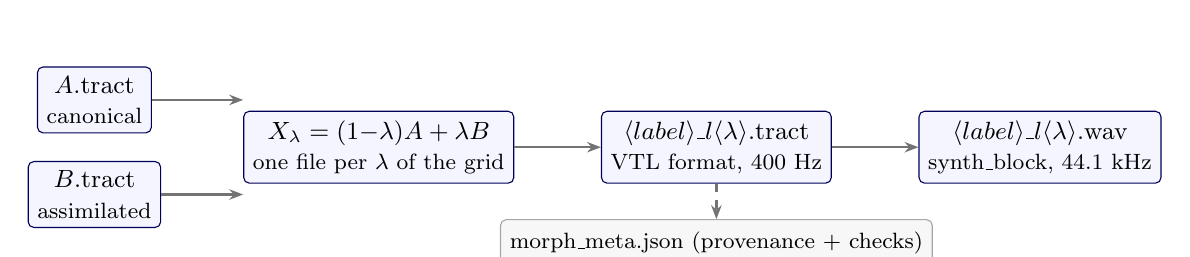
\begin{tikzpicture}[
  font=\small,
  box/.style={draw=blue!35!black, fill=blue!4, rounded corners=2pt,
              minimum height=0.75cm, align=center},
  side/.style={draw=black!35, fill=black!3, rounded corners=2pt,
               minimum height=0.6cm, align=center, font=\footnotesize},
  arr/.style={-{Stealth[length=5pt]}, thick, black!55}
]
  \node[box] (a) {$A.\text{tract}$\\{\footnotesize canonical}};
  \node[box, below=0.35cm of a] (b) {$B.\text{tract}$\\{\footnotesize assimilated}};
  \node[box, right=1.1cm of $(a.east)!0.5!(b.east)$, anchor=west] (blend)
        {$X_\lam = (1{-}\lam)A + \lam B$\\{\footnotesize one file per $\lam$ of the grid}};
  \node[box, right=1.1cm of blend] (tract) {$\langle label\rangle\_l\langle\lam\rangle.\text{tract}$\\{\footnotesize VTL format, 400 Hz}};
  \node[box, right=1.1cm of tract] (wav) {$\langle label\rangle\_l\langle\lam\rangle.\text{wav}$\\{\footnotesize synth\_block, 44.1 kHz}};
  \node[side, below=0.45cm of tract] (meta) {$\text{morph\_meta}.\text{json}$ (provenance + checks)};
  \draw[arr] (a.east) -- (blend.west |- a.east);
  \draw[arr] (b.east) -- (blend.west |- b.east);
  \draw[arr] (blend) -- (tract);
  \draw[arr] (tract) -- (wav);
  \draw[arr, dashed] (tract) -- (meta);
\end{tikzpicture}
\caption{The lambda-morph data path.  The dashed side output
records source hashes, the alignment report and the endpoint
identity checks of \sectref{sec:guarantees}.}
\label{fig:pipeline}
\end{figure}

Two properties make equation~\eqref{eq:morph} the right primitive
for articulatory continua.  First, it is \emph{exact at the
endpoints}: in IEEE-754 arithmetic $(1-0)A + 0B = A$ and
$(1-1)A + 1B = B$, so $\lam=0$ and $\lam=1$ do not degrade their
sources (this is asserted, not assumed; see
\sectref{sec:guarantees}).  Second, it is \emph{monotone and
linear in every parameter}, which gives the continuum a clean
articulatory reading: at $\lam = 0.5$ the lip-closure parameter LP
is exactly halfway between its canonical and assimilated values,
and the same holds for every column.  Intermediate stimuli are
articulatorily interpretable, not merely acoustically
intermediate.

\subsection{The frame-alignment contract}\label{sec:align}

The morph is \emph{spatial, never temporal}: it requires
$A$ and $B$ to have the same number of frames $T$ and the same
column layout, and it performs no time warping.  This is the
frame-alignment contract.  It holds by construction when the two
variants are cluster minimal pairs with the same segmental skeleton
--- same phonemes, same durations, a single phoneme substituted~---
such as \code{klinpan} versus \code{klimpan}: the engine's timers
are driven by segment counts and durations, which are identical, so
the two synthesis runs land on the same $T$ and the same event grid.

When the contract is violated, \code{check\_alignment} raises
\code{MorphAlignmentError} before anything is written.  When it
holds, the driver reports the \emph{divergence window}: the range of
frame indices on which the tract blocks differ.  Outside that window
the two sequences agree to machine precision and the blend is the
identity, which is the desired behaviour: the continuum must not
perturb the carrier material.  (In the target mode the corresponding
report is the \emph{measured footprint} of \sectref{sec:semantic},
bounded by the C1-incident arcs.)

\begin{keybox}[Frame alignment, operationally]
Two inputs are frame-aligned when they differ by
\emph{substitution} of phonemes (ideally one), not by insertion,
deletion or re-timing.  Safe recipes: cluster minimal pairs in
engine SAMPA (\code{klinpan}/\code{klimpan}~--- dotless; C.C splits
are out of scope, \sectref{sec:semantic}); or any two
\code{.tract} files verified with \code{check\_alignment}.  If a
glottis difference is reported, decide it explicitly with the
glottis policy below.
\end{keybox}

\subsection{Glottis policy}\label{sec:glottis}

The glottis block carries voicing, F0, and (via the nasal tag
envelope) nasality.  Blending it would confound the place-of-articulation
manipulation with source changes.  The option therefore makes the
policy explicit:

\begin{itemize}[leftmargin=1.6em]
\item \code{common} (default)~--- the glottis sequences of $A$ and
$B$ must be identical up to a tolerance ($10^{-6}$ by default,
configurable).  The morph then uses them unchanged: equation%
~\eqref{eq:morph} is a no-op on the glottis block, voicing and F0
contours are constant along the continuum, and the manipulation is
a pure tract operation.  A violation raises \code{MorphError} with
the measured maximal difference, steering the user to either fix
the inputs or opt into interpolation.
\item \code{interpolate}~--- the glottis block is blended with the
same weight.  Use it when the two variants genuinely differ in the
source (for example a voiced/voiceless pair), accepting that the
continuum then mixes both dimensions.
\end{itemize}

For the reference pairs the measured glottis difference is exactly
$0.0$: the engine derives both variants from the same segmental
skeleton, so the source columns agree bitwise.

\subsection{Guarantees}\label{sec:guarantees}

Every run computes and records its guarantee booleans in
\code{morph\_meta.json}.  The target mode (default, v1.2.0) records:

\begin{enumerate}[leftmargin=1.6em]
\item \code{lam0\_bitwise\_canon}~--- $\lam = 0$ reproduces the
canonical cluster synthesis (\code{vtl-synth run <phrase>})
bitwise (\code{np.array\_equal} on the full 30-column sequence);
\item \code{lam1\_theta\_equals\_c2}~--- the $\lam = 1$ item's C1
theta \emph{equals} $\theta_{C2}$ exactly (verbatim float;
\code{lam1\_rho\_equals\_c2} likewise with \code{--target-rho});
\item \code{glottis\_bitwise\_constant}~--- voicing, F0 and
nasality envelopes are bitwise identical at every $\lam$;
\item \code{outside\_c1\_arcs\_bitwise\_canon}~--- every frame
outside the C1-incident arcs (padded by one 100~Hz gesture sample
for the 100$\to$400~Hz upsampling) is bitwise canonical at every
$\lam$: C2 and the context never move.
\end{enumerate}

The blend mode records the v1.0/v1.1 set:
\begin{itemize}[leftmargin=1.6em]
\item \code{endpoint\_lam0\_equals\_canon} and
  \code{endpoint\_lam1\_equals\_assim} (or, with \code{confine},
  \code{confine\_lam1\_equals\_assim\_inside} and
  \code{outside\_confine\_equals\_canon});
\item \code{glottis\_noop\_at\_lam0} (common mode).
\end{itemize}

A failed check aborts the run: in exact arithmetic these identities
cannot fail (the weights are exact floats $0$ and $1$), so a
failure would indicate a numerical anomaly worth reporting.  The
\code{.wav} of an endpoint is likewise the deterministic
\code{synthesize\_audio} of the endpoint \code{.tract} content ---
the test suite pins this byte-for-byte
(\sectref{sec:tests}).

\begin{keybox}[One honest subtlety]
The morph operates on the \code{.tract} \emph{file representation},
whose text format quantizes parameters to six decimals.  The
$\lam=0$ output therefore reproduces the canonical \code{.tract}
file bitwise~--- not the in-memory float64 sequence that the
pipeline held before writing it.  The difference is at most
$5 \times 10^{-7}$ per parameter and is a property of the file
format, not of the morph.
\end{keybox}

\subsection{What the morph is not}

Three limitations delimit the option.  First, it is \emph{not a
time-warping tool}: inputs with different segmental skeletons must
be re-aligned upstream (the contract of \sectref{sec:align}).
Second, the interpolation is linear \emph{in the Maeda-type
parameter space} of VocalTractLab; it is not uniformly linear in
acoustic space, nor does it pass through any ``natural'' intermediate
gesture~--- the intermediate states are convex combinations, and
whether a given $\lam$ sounds like a good $[\text{n}]/[\text{m}]$
half-way token is an empirical question (exactly the question the
probing experiments ask).  Third, the option does not synthesize
endpoints itself in file mode: it consumes \code{.tract} files, so
the speaker, language and prosody of the endpoints are whatever
produced those files~--- which is also what makes the option
speaker-agnostic.

% ======================================================================
\section{Installing and removing the patch}\label{sec:install}
% ======================================================================

\subsection{Requirements}

The patch targets a \code{covtl-pipeline} checkout (v1.1.0 or later,
commit \code{1d15ed7} verified) with its Python dependencies
(\code{numpy}; \code{scipy} only for the WAV convenience path).  A
typical installation is \code{pip install .} inside the checkout, as
described by the pipeline's own \code{INSTALLATION.md}.  Audio
synthesis additionally requires the \code{vocaltractlab-cython}
wheel; without it, the option still runs with \code{--no-audio}
(and the non-VTL tests still pass).  The patch scripts themselves
use the standard library only.

\subsection{Applying: \code{patch/apply\_patch.py}}

\begin{lstlisting}[style=shell]
python patch/apply_patch.py [--pipeline-root DIR] [--force]
\end{lstlisting}

The script locates the pipeline root (explicit flag, environment
variable \code{COVTL\_PIPELINE\_ROOT}, \code{./covtl-pipeline}, or a
walk-up search), then performs three guarded steps.  First, it
copies the three module files to their destinations, byte-compiling
each:
\begin{itemize}[leftmargin=1.8em, itemsep=0pt]
\item \code{patch/files/core\_morphing.py} $\to$
\code{vtl\_synth/core/morphing.py};
\item \code{patch/files/cli\_morph\_cmd.py} $\to$
\code{vtl\_synth/cli/morph\_cmd.py};
\item \code{patch/files/test\_morphing.py} $\to$
\code{tests/test\_morphing.py}.
\end{itemize}
Second, it patches
\code{vtl\_synth/cli/main.py}: the anchor line

\begin{lstlisting}[style=plain]
    # ---- global options (before the subcommand on the command line) ----
\end{lstlisting}

must occur exactly once~--- the script asserts it and aborts without
writing otherwise~--- and the insertion of
\sectref{sec:intro} is placed just before it, inheriting the file's
line endings (the shipped \code{main.py} uses CRLF; the insertion is
EOL-safe in both directions).  The original file is backed up to
\code{main.py.lambda-morph.bak}.  Third, it verifies the result by
byte-compiling \code{main.py} and probing, in a subprocess, that
\code{build\_parser()} now exposes the \code{morph} subcommand.
The applied insertion is exactly:

\begin{lstlisting}[style=python]
    # ---- morph (lambda-morph option, covtl-lambda-patch) ---------------
    # 2026-10-22: articulatory interpolation continuum option;
    # 2026-10-26: v1.2.0 semantic -- the lambda variation acts on
    # the tautosyllabic CC cluster C1C2 -> C1'C2: --targets moves
    # the C1 polar target (theta, optionally rho) toward the C2
    # target; the two-endpoint tract blend remains available.
    # Additive option -- no existing subcommand is modified.
    # Implementation: vtl_synth/core/morphing.py
    # + vtl_synth/cli/morph_cmd.py; tests: tests/test_morphing.py.
    # Apply/revert: patch/apply_patch.py, patch/revert_patch.py.
    from vtl_synth.cli.morph_cmd import add_morph_subparser
    add_morph_subparser(sub, _add_engine_options)
\end{lstlisting}

The script is idempotent: re-running it on a patched tree exits with
code~2 and a clear message (\code{--force} re-copies the module
files; the \code{main.py} insertion stays guarded by its own
marker).

\subsection{Removing: \code{patch/revert\_patch.py}}

\begin{lstlisting}[style=shell]
python patch/revert_patch.py [--pipeline-root DIR] [--keep-modules]
\end{lstlisting}

Reversion tries two strategies in order: restore \code{main.py}
from the backup written at apply time; or, if the backup is gone,
remove the insertion block by its comment markers with an
EOL-agnostic regular expression.  It then deletes the three added
files (unless \code{--keep-modules} is given, for users who want to
keep calling the Python API), byte-compiles \code{main.py} and
reports.  Other engine patches~--- for instance the \code{/N/}
closure patch in \code{constants.py}~--- are never touched.  After a
revert, the SHA-256 of \code{main.py} is byte-identical to its
pre-patch value (verified during the release tests).

\subsection{Non-regression statement}

The patch is \emph{additive}.  It adds three files and one guarded
insertion that only registers a new subcommand; no existing code
path, default, file format or output changes.  The engine's
regression baselines (\code{regression\_baselines*.json}) are
unaffected, and \code{vtl-synth run}, \code{text-to-wav},
\code{inspect}, \code{plot-tract}, the polar and prosody options
all behave exactly as before~--- importing \code{morphing.py}
executes no engine code (it only imports constants).

% ======================================================================
\section{Command-line reference}\label{sec:cli}
% ======================================================================

\subsection{Synopsis}

\begin{lstlisting}[style=shell]
# target mode (DEFAULT semantic, v1.2.0): one cluster phrase
vtl-synth morph --phonetic --targets PHRASE [-o DIR] [--label NAME]
    [--lambdas LIST | --n-steps N] [--target-rho] [--cluster N]
    [--no-audio] [engine options]

# blend mode (option): two endpoints
vtl-synth morph A B [-o DIR] [--label NAME]
    [--lambdas LIST | --n-steps N] [--glottis {common,interpolate}]
    [--tol TOL] [--confine T1:T2 | --confine-frames F1:F2] [--ramp N]
    [--no-audio] [--text] [engine options]
\end{lstlisting}

In the target mode \code{PHRASE} is the \emph{canonical cluster}
phrase in engine SAMPA, dotless (\code{klinpan}, \code{klinkan},
\code{minbot}~...): the option locates the nasal-initial CC cluster
(its C1 and C2 polar targets are read from the engine's own
syllabic build), interpolates the C1 target per $\lam$ and
re-synthesizes.  A phrase carrying a syllable dot is rejected
(C.C splits are out of scope, \sectref{sec:semantic}).

In the blend mode \code{A} is the canonical variant and \code{B}
the assimilated one.  Each argument is either a \code{.tract} file
(file mode, when the name ends with \code{.tract}) or a phrase
(phrase mode); the two must be of the same kind.  In phrase mode the
inputs are engine SAMPA by default~--- \code{klinpan},
\code{klimpan}~--- and the option synthesizes both endpoints first,
with \emph{identical} engine settings, in \code{<out>/\_endpoints/};
pass \code{--text} to run English text through the g2p instead
(assimilated spellings like \emph{cleam} are usually not in the
lexicon, and g2p output carries syllable dots, so SAMPA is the
recommended input for the lambda variation).

Table~\ref{tab:options} lists the options; the engine options
(\code{-s}, \code{-l}, \code{--tcons}, \ldots) are the standard
ones of \code{vtl-synth run} and apply to the synthesis of the
target-mode continuum (or of the two blend-mode endpoints).

\begin{table}[t]
\centering\small
\caption{Options of the \code{morph} subcommand.}\label{tab:options}
\begin{tabularx}{\textwidth}{@{}l l >{\raggedright\arraybackslash}X@{}}
\toprule
Option & Default & Description \\
\midrule
\code{-o}, \code{--output-dir} & \code{morph\_out} & destination of
the continuum files and of \code{morph\_meta.json}. \\
\code{--label} & derived & file stem of the items
(\code{<label>\_l<lam>.tract}); default \code{<A>-vs-<B>} in blend
mode, the phrase in target mode. \\
\code{--lambdas} &~--- & comma-separated weights in $[0,1]$, e.g.
\code{0,0.25,0.5,0.75,1}; deduplicated, sorted. \\
\code{--n-steps} & 9 & uniform grid of $N \ge 2$ steps from 0 to 1
inclusive. \\
\code{--targets} & off & \textbf{default semantic} (v1.2.0):
single-phrase target morph on the CC cluster
(\sectref{sec:semantic}); \code{B} must be absent. \\
\code{--target-rho} & off & target mode: also interpolate the C1
rho toward the C2 rho (default: theta only). \\
\code{--cluster} & 1 & target mode: 1-based rank of the
nasal-initial CC cluster when the phrase carries several. \\
\code{--glottis} & \code{common} & blend-mode glottis policy of
\sectref{sec:glottis} (target mode: bitwise constant by
construction). \\
\code{--tol} & \code{1e-6} & tolerance of the \code{common} glottis
identity check. \\
\code{--confine} / \code{--confine-frames} & whole sequence &
blend mode: restrict the blend to the C1 window (seconds or 400~Hz
frames); context held canonical at every $\lam$. \\
\code{--ramp} & 10 & raised-cosine edge ramp of the confine window
(frames). \\
\code{--no-audio} & off & write the \code{.tract} continuum only. \\
\code{--text} & off & blend-mode phrase inputs are English text
(g2p) instead of SAMPA. \\
\bottomrule
\end{tabularx}
\end{table}

\subsection{A worked session}

\begin{lstlisting}[style=shell]
$ vtl-synth morph --phonetic --targets klinpan -o out/P1 --label P1
[morph] mode      : targets (C1C2 -> C1'C2 on the tautosyllabic cluster -- DEFAULT semantic, v1.2.0)
[morph] label     : P1
[morph] frames    : 584 @ 400 Hz
[morph] cluster   : C1 n (rho 1.150, theta 4.7124 rad) -> C2 p (rho 1.060, theta 0.8727 rad); dtheta +140.00 deg, theta only
[morph] C1 window : frames 232-271 (phoneme span); C1-incident arcs frames 232-311
[morph] footprint : frames 229-307 (measured, all lambdas vs canon)
[morph] check     : lam0_bitwise_canon = True
[morph] check     : glottis_bitwise_constant = True
[morph] check     : lam1_theta_equals_c2 = True
[morph] check     : outside_c1_arcs_bitwise_canon = True
[morph] lambda=0  theta_C1=+4.712389 rad  out/P1/P1_l0.tract  + out/P1/P1_l0.wav
[morph] lambda=0.125  theta_C1=+5.017822 rad  out/P1/P1_l0.125.tract  + out/P1/P1_l0.125.wav
    (seven further rows, one per lambda of the grid, omitted)
[morph] lambda=1  theta_C1=+0.872665 rad  out/P1/P1_l1.tract  + out/P1/P1_l1.wav
[morph] meta      : out/P1/morph_meta.json
\end{lstlisting}

The four \code{check} lines are the guarantees of
\sectref{sec:guarantees}; the \code{footprint} line is the measured
divergence extent of all $\lam$ against the canonical cluster,
bounded by the C1-incident arcs.  A dotted phrase fails early with
an explanatory error, as does a phrase without a nasal-initial
cluster.

% ======================================================================
\section{Python API reference}\label{sec:api}
% ======================================================================

All entry points live in \code{vtl\_synth.core.morphing}.  Two
exceptions signal misuse: \code{MorphError} (itself a
\code{ValueError}) and its subclass \code{MorphAlignmentError},
raised on frame-count and layout mismatches.

\begin{table}[t]
\centering\small
\caption{Public API of \code{vtl\_synth.core.morphing}.}\label{tab:api}
\begin{tabularx}{\textwidth}{@{}>{\raggedright\arraybackslash}p{5.9cm} >{\raggedright\arraybackslash}X@{}}
\toprule
Symbol & Role \\
\midrule
\code{morph\_targets(phrase, output\_dir, ...)} & driver (DEFAULT
semantic): cluster phrase $\to$ continuum of re-synthesized
\code{.tract} (+ \code{.wav}) + \code{morph\_meta.json}. \\
\code{build\_target\_continuum(phrase, ...)} & arrays: per-$\lam$
rebuilt cluster (tract + glottis), plan, checks, footprint. \\
\code{plan\_target\_cluster(phrase, ...)} & locates the C1C2
cluster: C1/C2 polar targets, $\Delta\theta$, C1 windows; rejects
dotted phrases. \\
\code{find\_nasal\_c1\_clusters(nodes)} & nasal-initial
tautosyllabic CC clusters of a syltraj node list. \\
\code{interp\_target\_theta/rho(th1, th2, lam)} & the target rule
\eqref{eq:target} with exact (verbatim) endpoints;
\code{wrap\_angle\_delta} is the shortest-path difference. \\
\code{morph\_pair(canon, assim, output\_dir, ...)} & blend-mode
driver: files $\to$ continuum of \code{.tract} (+ \code{.wav}) +
\code{morph\_meta.json}. \\
\code{build\_continuum(A, B, lambdas, ...)} & blend-mode arrays
$\to$ \code{ContinuumResult} (items, \code{AlignmentReport},
checks). \\
\code{interpolate\_tract(A, B, lam)} & the raw blend rule
\eqref{eq:morph} with shape and range guards. \\
\code{check\_alignment(A, B)} & shapes/glottis/divergence-window
report; raises on misalignment. \\
\code{confine\_weight(n, first, last, ramp)} & raised-cosine window
of the blend-mode confine. \\
\code{parse\_lambda\_grid(spec, n\_steps)} & grid parsing/validation
($[0,1]$, dedup, sort). \\
\code{read\_tract\_sequence(path)} & \code{.tract} $\to$
\code{(data, sr)}; \code{write\_morph\_tract(path, data, sr)} writes
the canonical VTL header. \\
\code{window\_state(data, t0, t1, mode)} & articulatory ground
truth in a time window (\code{mid} frame or \code{mean}). \\
\code{MORPH\_GLOTTIS\_MODES}, \code{DEFAULT\_N\_STEPS},
\code{DEFAULT\_GLOTTIS\_TOL}, \code{NASAL\_C1\_KEYS} & module
constants. \\
\bottomrule
\end{tabularx}
\end{table}

\subsection{Driving a continuum from Python}

\begin{lstlisting}[style=python]
from vtl_synth.core.morphing import morph_targets, morph_pair

# the DEFAULT semantic (v1.2.0): one cluster phrase, polar targets
meta = morph_targets(
    'klinpan',                                # canonical cluster
    output_dir='work/lambda/P1',
    lambdas=[0.0, 0.125, 0.25, 0.375, 0.5, 0.625, 0.75, 0.875, 1.0],
    rho_enabled=False,                        # or True: theta + rho
    label='P1')
print(meta['targets'])   # C1/C2 targets, dtheta, C1 windows
print(meta['checks'])    # lam0 canon, lam1 theta == C2, glottis,
                         # outside-C1-arcs canonical (all True)

# option: the two-endpoint tract blend (v1.0/v1.1 semantics)
meta = morph_pair(
    'work/base/P1_canon/P1_canon.tract',   # canonical endpoint
    'work/base/P1_assim/P1_assim.tract',    # assimilated endpoint
    output_dir='work/lambda/P1',
    lambdas=[0.0, 0.125, 0.25, 0.375, 0.5, 0.625, 0.75, 0.875, 1.0],
    glottis_mode='common',
    confine=(232, 272),
    label='P1')
\end{lstlisting}

Existing \code{.wav} files are not re-synthesized unless
\code{overwrite=True} is passed, so a failed downstream stage can
resume where the synthesis stopped~--- the same convention as the
kit experiment the option comes from.

\subsection{The \code{morph\_meta.json} record}

\begin{table}[t]
\centering\small
\caption{Schema of \code{morph\_meta.json} (target mode).  The blend
mode of v1.0/v1.1 replaces \code{targets}, \code{engine} and
\code{diff\_extent\_frames} with \code{sources}, \code{glottis\_mode},
\code{alignment} and \code{confine}.}\label{tab:meta}
\begin{tabularx}{\textwidth}{@{}l X@{}}
\toprule
Key & Content \\
\midrule
\code{patch}, \code{mode} & patch identity string; \code{targets}
(or \code{blend}). \\
\code{label}, \code{phrase} & item stem; the canonical cluster
phrase (normalized engine input). \\
\code{semantic} & one-line statement of the v1.2.0 semantic. \\
\code{targets} & C1/C2 keys and polar targets, $\Delta\theta$
(rad and deg), \code{rho\_enabled}, the C1 phoneme window and the
C1-incident-arcs window (400~Hz frames). \\
\code{engine} & (co)articulation parameters actually used (speaker,
f0, gesture timings, orthogonal branch). \\
\code{lambdas} & the grid, as floats. \\
\code{diff\_extent\_frames} & measured footprint of all $\lam$
against the canonical cluster. \\
\code{checks} & the guarantee booleans of \sectref{sec:guarantees}. \\
\code{items} & one record per $\lam$: weight, the
$\lam$-interpolated C1 target (\code{theta\_c1}, optionally
\code{rho\_c1}), \code{.tract} path, \code{.wav} path (or
\code{null}), frame count. \\
\bottomrule
\end{tabularx}
\end{table}

The record is deliberately self-contained: together with the two
hashed sources it is enough to re-derive every continuum file, and
to audit that a reported stimulus set really is the convex
combination it claims to be.

% ======================================================================
\section{The assimilation continuum, end to end}\label{sec:experiment}
% ======================================================================

\subsection{The reference experiment}

The example shipped with the patch
(\code{examples/lambda\_continuum.py}) reproduces the synthesis side
of the original lambda experiment under the v1.2.0 target semantic.
Two cluster pairs are built from engine SAMPA with default settings
(speaker jd3, 100/80/200~ms timings):

\begin{table}[t]
\centering\small
\caption{The reference pairs (tautosyllabic clusters, dotless).
\emph{Licensed} refers to the phonological licensing of the
assimilation: place agreement with the following stop is licit
before a labial, illicit before an alveolar.  The assimilated
endpoint is not a second phrase: at $\lam=1$ the C1 polar target
has reached the C2 target.}\label{tab:pairs}
\begin{tabularx}{\textwidth}{@{}l l l l X@{}}
\toprule
Pair & Canonical cluster & C2 & Licensing & Transition \\
\midrule
P1 & \code{klinpan} & /p/ & licensed &
$\theta_{C1}: 270^\circ \to 50^\circ$ ($+140^\circ$) \\
NV1 & \code{klintan} & /t/ & unlicensed &
$\theta_{C1}: 270^\circ \to -75^\circ$ ($+15^\circ$) \\
\bottomrule
\end{tabularx}
\end{table}

Each pair is built on the nine-step grid
$\{0, 0.125, \ldots, 1\}$; the articulatory ground truth is read at
the C1 target window 0.58--0.68~s (mid frame 0.63~s) with
\code{window\_state}.  Running the example takes a few minutes and
prints, per pair, the cluster targets, the guarantee checks and the
articulator table of Table~\ref{tab:articulators}.

\begin{table}[t]
\centering\small
\caption{Articulatory ground truth along the continuum (pair P1,
$t = 0.63$~s, mid of the C1 arrival arc): lip proximity LP, lip
distance LD, jaw angle JA (degrees) and velum opening VO, in engine
units.}\label{tab:articulators}
\begin{tabular}{@{}rrrrr@{}}
\toprule
$\lam$ & LP & LD & JA & VO \\
\midrule
0      & 0.177 & 0.645 & $-2.321$ & 0.886 \\
0.125  & 0.177 & 0.645 & $-2.181$ & 0.886 \\
0.25   & 0.177 & 0.645 & $-2.126$ & 0.886 \\
0.375  & 0.177 & 0.645 & $-2.162$ & 0.886 \\
0.5    & 0.177 & 0.645 & $-2.285$ & 0.886 \\
0.625  & 0.177 & 0.645 & $-2.484$ & 0.886 \\
0.75   & 0.177 & 0.645 & $-2.740$ & 0.886 \\
0.875  & 0.177 & 0.645 & $-3.030$ & 0.886 \\
1      & 0.177 & 0.645 & $-3.327$ & 0.886 \\
\bottomrule
\end{tabular}
\end{table}

The table reads as the anatomy of the target morph at mid-arc.
The velum stays wide open (VO constant at 0.886): the continuum
remains a nasal throughout~--- C1 keeps its nasal identity
(selector, nasality envelope) while its \emph{target} rotates
toward the C2 place.  At the mid-arc probe the place change is
carried by the jaw and the tongue (JA falls by about one degree;
TTX/TTY move monotonically, cf.\ Figure~\ref{fig:data}), while the
lips still follow the vowel background (LP/LD constant to three
decimals at this frame; the labial closure emerges along the
second half of the arc).  Unlike the blend mode these values are
\emph{not} linear in $\lam$: they follow the engine's arc geometry
(the raised-cosine mixing of departure and arrival targets), which
is exactly the point~--- the continuum is a family of
re-synthesized clusters, not a convex combination of two
recordings.

\subsection{Reading the figure}

Figure~\ref{fig:data} shows the same data as time series and as
ground-truth curves.

\begin{figure}[t]
\centering
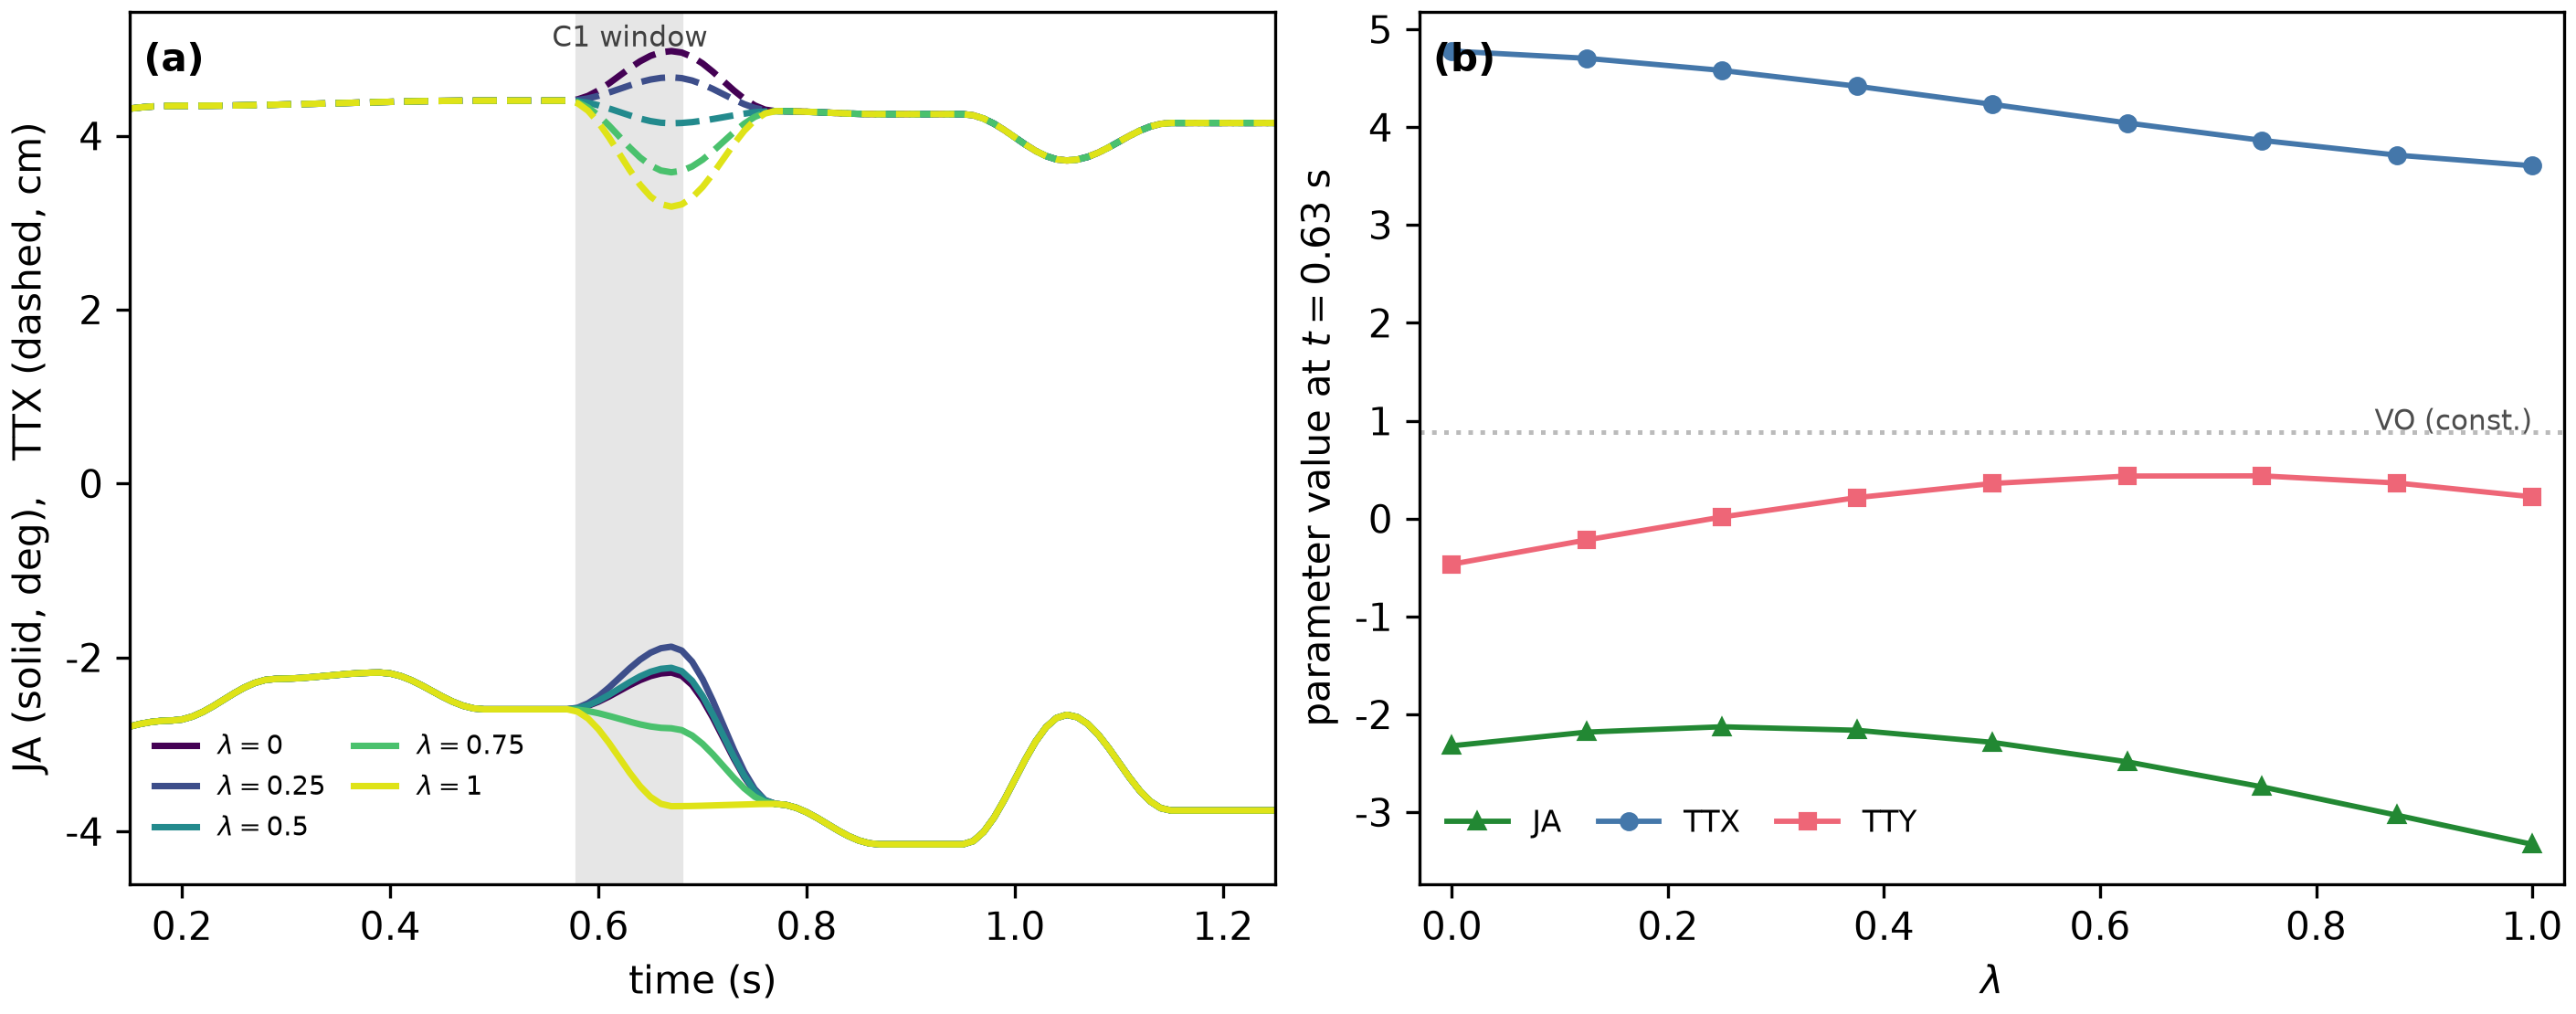
\includegraphics[width=\textwidth]{figures/fig_continuum_data.png}
\caption{The P1 target continuum.  (a)~The articulators that carry
the place change~--- jaw angle JA (solid) and tongue-tip x TTX
(dashed)~--- over time for five weights of the grid (viridis ramp
from $\lam=0$ dark purple to $\lam=1$ yellow); the shaded band is
the 0.58--0.68~s C1 window.  Outside the C1-incident arcs all
curves superpose bitwise: the context (C2 /p/ included) never
moves.  (b)~Articulatory ground truth at $t = 0.63$~s against
$\lam$: JA, TTX, TTY follow the arc geometry; VO is constant
(dotted).}\label{fig:data}
\end{figure}

Panel~(a) makes the locality of the manipulation visible: the five
JA trajectories share their onset and offset gestures and fan apart
only inside the C1-incident arcs (the arrival arc into the nasal
and the nasal$\to$/p/ arc), re-merging before the following vowel;
the TTX curves mirror them.  The shaded band marks where downstream
analyses should read the articulatory state.  Panel~(b) shows the
arc-geometry response of the three moving articulators and the flat
nasality line~--- a pure place-of-articulation dial with the
nasality valve left alone.

\subsection{Relation to the source experiment}

The option generalizes the kit's stage~A lambda experiment, with
one semantic correction: the kit synthesized \emph{dotted} forms
(\code{klin.pan}/\code{klim.pan}, C.C splits) and blended the two
endpoint tracts; the v1.2.0 semantic operates on the
\emph{tautosyllabic cluster} (\code{klinpan}) and its polar targets,
which is the object the assimilation process actually acts on
(\sectref{sec:semantic}).  The dotted blend remains reproducible
with the blend mode on any frame-aligned pair, but it is no longer
the documented semantic of the lambda variation; the kit's recorded
dotted-stage values (LP $0.214 \to 0.742$, divergence frames
97--307) belong to that legacy path.  The cluster example serves as
the regression anchor of the target semantic: any future change in
the engine's trajectory machinery that shifts the continuum (or the
C1 windows) will surface here first.

% ======================================================================
\section{Testing and guarantees}\label{sec:tests}
% ======================================================================

The patch ships \code{tests/test\_morphing.py}~--- 53~tests in three
layers, runnable from the pipeline root with
\code{python -m pytest tests/test\_morphing.py -q}.  The pure-numpy
layer (no VocalTractLab required) covers the blend interpolation
identities (bitwise endpoints, exact midpoint), the grid parser
(specs, uniform steps, out-of-range and malformed rejections), the
alignment report (divergence window, glottis reporting), the glottis
policies (rejection under \code{common}, blending under
\code{interpolate}), the \code{.tract} write/read round trip with
its six-decimal quantization, the \code{window\_state} helper, the
\code{morph\_pair} driver without audio (file naming, metadata
schema, mutual exclusion of grid arguments, confine records), the
CLI parser wiring, and the pure target arithmetic (shortest-path
angle wrap, verbatim endpoint identity of
\code{interp\_target\_theta}/\code{interp\_target\_rho}).  The
engine-core layer (syltraj available, no VTL wheel) plans real
cluster phrases: nasal-cluster detection on the six Pouw pairs
(onset clusters correctly skipped), dotted-phrase rejection,
C1/C2 target values, C1 windows and their engine-override shift.
The VTL-gated layer synthesizes end to end: the target continuum
guarantees of \sectref{sec:guarantees} on \code{klinpan}/%
\code{klinkan} (including the rho channel), the
\code{morph\_targets} driver and metadata, the blend-mode
subcommand, and the determinism pin: the \code{.wav} of $\lam=0$ is
byte-identical to a direct \code{synthesize\_audio} of the
canonical \code{.tract} content, while genuinely differing from
the $\lam=1$ output.

\begin{table}[t]
\centering\small
\caption{Test inventory (53 tests).}\label{tab:tests}
\begin{tabularx}{\textwidth}{@{}l l X@{}}
\toprule
Layer & Count & What is pinned \\
\midrule
Grids & 8 & default 9 steps; spec parse/dedup; $N$-step grids;
range and format rejections (parametrized); $N \ge 2$. \\
Blend identities & 4 & bitwise $\lam=0$/$\lam=1$; exact midpoint;
shape-mismatch and range guards. \\
Alignment + glottis & 7 & report fields and divergence window;
frame-count mismatch; \code{common} rejection /
\code{interpolate} blending; checks recorded; unknown mode;
mode constants. \\
I/O & 1 & \code{.tract} round trip (header, 6 decimals). \\
Ground truth & 3 & mid-frame selection; window mean; mode guard. \\
Blend driver & 3 & continuum + meta on disk; grid-argument
exclusivity; default label and grid. \\
Confine (v1.1.0) & 7 & weight shape/bounds/rejection/clamping;
context-canonical guarantee; hard window at ramp 0; legacy
unconfined behaviour; confine recorded in meta. \\
CLI parser & 2 & blend wiring; \code{--targets}/%
\code{--target-rho}/\code{--cluster} flags, single-phrase
invocation. \\
Blend VTL & 2 & file-mode subcommand end to end; endpoint WAV
determinism. \\
Target arithmetic & 4 & angle wrap; verbatim theta endpoints;
verbatim rho endpoints; nasal key set. \\
Target planning & 6 & nasal clusters on the six Pouw pairs; dotted
forms are not clusters; plan semantics + windows; dotted rejection;
clusterless rejection; engine-override window shift. \\
Target synthesis (VTL) & 4 & continuum guarantees; rho channel;
driver + meta; CLI end to end. \\
Target CLI rejections & 2 & dotted phrase; two-input misuse. \\
\bottomrule
\end{tabularx}
\end{table}

% ======================================================================
\section{Limitations and extensions}\label{sec:limits}
% ======================================================================

Three directions delimit the current design and sketch its natural
extensions.  First, the blend mode's frame-alignment contract
excludes pairs that differ in segmental content~--- one cannot
blend \emph{clean pan} into \emph{cleanly pan} without an upstream
alignment stage; the target mode has no such constraint (one phrase
in), but it is defined on nasal-initial CC clusters only, and on
the two target channels $\theta$ (always) and $\rho$
(optionally)~--- interpolating further properties of the C1 gesture
(selector set, nasality envelope) would be a semantic extension,
deliberately not offered.  Second, the target interpolation is
linear in the polar angle along the shortest arc; exotic contexts
where the articulatorily natural route is the long way around would
need an orientation option.  Third, the option currently outputs
\code{.tract}/\code{.wav} pairs; feeding the continuum directly
into the video or probing layers is left to composition~--- the
metadata record (which now carries the per-item C1 target) is
designed to be the glue.

% ======================================================================
\begin{thebibliography}{9}\label{sec:refs}
% ======================================================================

\bibitem{pouw2024}
C.~Pouw, M.~de~Heer~Kloots, A.~Alishahi, and W.~Zuidema.
\newblock Perception of phonological assimilation by neural speech
  recognition models.
\newblock \emph{Computational Linguistics}, 50(4):1557--1585, 2024.

\bibitem{berthommier2021}
F.~Berthommier, ``A mathematical model of the vowel space,''
arXiv:2111.00868 [eess.AS], 2021.

\bibitem{berthommier2023}
F.~Berthommier, ``Why can big.bi be changed to bi.gbi?~A
mathematical model of syllabification and articulatory synthesis,''
arXiv:2307.02299 [eess.AS], 2023.

\bibitem{berthommier2024}
F.~Berthommier, ``Synth\`ese de syllabes avec un mod\`ele de Maeda
pilot\'e par une repr\'esentation complexe,'' in \emph{Actes des
35\`emes Journ\'ees d'\'Etudes sur la Parole (JEP)}, pp.~541--550,
ATALA/AFPC, 2024.

\bibitem{birkholz}
P.~Birkholz, ``Modeling consonant-vowel coarticulation for
articulatory speech synthesis,'' \emph{PLoS ONE}, 8(4):e60603,
2013. VocalTractLab 2.4: \url{https://www.vocaltractlab.de}.

\bibitem{gaskell1996}
M.~G.~Gaskell and W.~D.~Marslen-Wilson.
\newblock Phonological variation and inference in lexical access.
\newblock \emph{Journal of Experimental Psychology: Human Perception and
  Performance}, 22(2):327--342, 1996.

\bibitem{krug}
P.~Krug, VocalTractLab-Python (vocaltractlab-cython).
\url{https://github.com/paul-krug/VocalTractLab-Python}.

\bibitem{nasalkit}
covtl-lambda-patch contributors, \emph{nasal\_synthesis
reproducibility kit} (internal), 2026: the wav2vec2 probing and
lambda-continuum study this option was extracted from.

\end{thebibliography}

\hypersetup{
    pdftitle={The Lambda-Morph Option for covtl-pipeline},
    pdfauthor={covtl-lambda-patch contributors},
    pdfsubject={Articulatory interpolation continua between frame-aligned utterances},
    pdfkeywords={articulatory synthesis, morphing, interpolation continuum, assimilation, VocalTractLab, COVTL}
}

\end{document}
